\documentclass[12pt]{llncs}



% This is LLNCS.DEM the demonstration file of
% the LaTeX macro package from Springer-Verlag
% for Lecture Notes in Computer Science,
% version 2.4 for LaTeX2e as of 16. April 2010
%
%

% ADDED CUSTOM PACKAGES
% Fonts
\usepackage{mathptmx}
% Layout
\usepackage[margin=20mm]{geometry}
\usepackage{setspace}
\doublespacing
\usepackage{multicol}
\usepackage{bbm}
\usepackage{url}
\bibliographystyle{splncs03}


\usepackage{amssymb,array}
\usepackage{enumitem}


% Maths
\usepackage{amsmath}
\newcommand*\diff{\mathop{}\!\mathrm{d}}
\newcommand*\Diff[1]{\mathop{}\!\mathrm{d^#1}}
\usepackage{algorithm}
\usepackage{algpseudocode}


% Graphics
\usepackage{placeins}
\usepackage{graphicx}
% \graphicspath{{../../Papers/ECML/Images/}}
\usepackage{caption}
\captionsetup{compatibility=false}
\usepackage{subcaption}
\usepackage{tikz} % Essential for Neural Network diagrams



\tikzstyle{state}=[shape=circle,draw=blue!50,fill=blue!20]
\tikzstyle{observation}=[shape=rectangle,draw=orange!50,fill=orange!20]
\tikzstyle{lightedge}=[<-,dotted]
\tikzstyle{mainstate}=[state,thick]
\tikzstyle{mainedge}=[<-,thick]


\usepackage[colorlinks=true,linkcolor=blue,urlcolor=black, bookmarksdepth=2]{hyperref}
\usepackage{bookmark}
\usepackage{comment}
% Custom environments

\newenvironment{Figure}
  {\par\medskip\noindent\minipage{\linewidth}}
  {\endminipage\par\medskip}

%\usepackage{natbib}   
%\newcommand{\citep}{\cite} % remove me when the natbib issue is resolved
%\newcommand{\citet}{\cite} % remove me when the natbib issue is resolved
%\newcommand{\citeyear}[1]{YEAR } % remove me when the natbib issue is resolved

% END CUSTOM PACKAGES

\usepackage{makeidx}  % allows for indexgeneration
\usepackage[draft]{todonotes}
\setlength{\marginparwidth}{1.5cm} % Not a lot of space for notes in margin
% dav's notes
\newcommand{\dzN}[1]{\todo[inline, size=\small, color=yellow!30]{[dz] #1}}
\newcommand{\dzn}[1]{\todo[color=yellow!30]{[dz] #1}}
% ivan's notes
\newcommand{\ikN}[1]{\todo[inline, size=\small, color=orange!30]{[ik] #1}}
\newcommand{\ikn}[1]{\todo[size = \small, color=orange!30]{[ik] #1}}
% steve's notes
\newcommand{\srN}[1]{\todo[inline, size=\small, color=cyan!30]{[sr] #1}}
\newcommand{\srn}[1]{\todo[color=cyan!30]{[sr] #1}}
% ber's notes
\newcommand{\bpN}[1]{\todo[inline, size=\small, color=purple!30]{[bp] #1}}
\newcommand{\bpn}[1]{\todo[color=purple!30]{[bp] #1}}
% theo's notes
\newcommand{\twN}[1]{\todo[inline, size=\small, color=green!30]{[tw] #1}}
\newcommand{\twn}[1]{\todo[color=green!30]{[tw] #1}}
% yunpeng's notes
\newcommand{\ylN}[1]{\todo[inline, size=\small, color=blue!30]{[yl] #1}}
\newcommand{\yln}[1]{\todo[color=blue!30]{[yl] #1}}

% ms's notes
\newcommand{\msN}[1]{\todo[inline, size=\small, color=gray!30]{[ms] #1}}
\newcommand{\msn}[1]{\todo[color=gray!30]{[ms] #1}}

\begin{document}
%
%\setcounter{tocdepth}{4}
%\tableofcontents


%
\pagestyle{headings}  % switches on printing of running heads

%
\mainmatter              % start of the contributions


\title{Signal Detection with Deep Learning and Kernel Methods}
%

%\titlerunning{Hamiltonian Mechanics}  % abbreviated title (for running head)
%                                     also used for the TOC unless
%                                     \toctitle is used
%
\author{Ivan Kiskin\inst{1,2}}
%
% \authorrunning{Ivar Ekeland et al.} % abbreviated author list (for running head)
%
%%%% list of authors for the TOC (use if author list has to be modified)
% \tocauthor{Ivar Ekeland, Roger Temam, Jeffrey Dean, David Grove,
% Craig Chambers, Kim B. Bruce, and Elisa Bertino}
%
\institute{University of Oxford, Department of Engineering, Oxford OX1 3PJ, UK, \\
\and
\email{\textrm{ikiskin@robots.ox.ac.uk}}, 
}
% \and
% \email{\textrm{\{}ikiskin, ber, dzilli, sjrob\textrm{\}}@robots.ox.ac.uk}, 
% % \and
% % \email{ber@robots.ox.ac.uk}\\
% \institute{test, \\
% \and
% \email{theo.windebank@stcatz.ox.ac.uk}}\\
% \and
% \email{dzilli@robots.ox.ac.uk}\\
% \and
% \email{marianne.sinka@zoo.ox.ac.uk}
% % \and
% \email{sjrob@robots.ox.ac.uk}
%\and
%\institute{University of Oxford, Department of Zoology, Oxford OX2 6GG, UK}}


\maketitle              % typeset the title of the contribution




\ikN{General notes: \\
Title sucks\\
Certain proposed lines of work in the proposal section could benefit from a literature review in those suggested fields. E.g.: \\
 Have not spoken about wavelets at all in literature review.}
\section{Introduction}

Signal detection is a very broad research area with contributions from a wide range of academic disciplines. We define signal detection as the ability to discern information-bearing patterns from random patterns that contain no information. The aim of the DPhil is to progress the state of the art by advancing real-world applications.  The motivation to excel in applications aligns with the need to innovate algorithms and architectures.

The literature review critically covers contributions to signal processing from deep learning in the context of speech detection, image recognition, and acoustic event detection. The research is examined in chronological order, following the progression of the state of the art in specific fields. We narrow down our focus to audio signals and images and highlight the potential areas in need of further improvements\ikn{Need to do this}, forming the basis of our research efforts. Section \ref{sec:speechrecognition} focuses on the speech recognition field, due to its competitive nature and associated rich publication record, as well as due to its similarity to our chosen application domains.\ikn{Which are?} The progress in state-of-the-art speech recognition was fuelled by both industry and academia due to its importance in human-machine interaction systems, that arguably are essential to general artificial intelligence \cite{rabiner1993fundamentals}, \cite{juang2005automatic}.

Section \ref{sec:imagerecognition} focuses on image recognition, the most competitive field in recent years due to the multitude of established image recognition and object detection challenges (with over 50 participating institutions by 2014 in the ImageNet Large Scale Visual Recognition Challenge alone \cite{russakovsky2014imagenet}). As a result, innovations have become influential to related fields in the scientific literature.
Our focus then shifts to bird species recognition and acoustic event detection in Sections \ref{sec:birdrecognition} and \ref{sec:AED} as fields where innovation was driven by progress in both speech and image recognition.

% We further highlight detection methods from traditional signal  processing literature  that show most potential promise of transferability to our application in Section  \ref{sec:traditional}.

\emph{Finally, we outline how reviewed methodology directly applies to our application of mosquito detection, which falls within the scope of noisy audio signal detection.} \ikn{To do}

The literature review is followed by the research proposal which includes a concise summary of completed work, future work, and a risk assessment. Future work is broken down into short, medium and long-term goals in Section \ref{sec:proposal}. We conclude with .... in Section \ref{sec:conclusion}.



\section{Speech Recognition}
\label{sec:speechrecognition}
Due to its significance in academia and industry, great attention is devoted to the field of speech recognition. Speech recognition has been a prominently researched field due to its critical role in human-machine interactions. The ability to accurately transcribe spoken text would influence a diverse range of applications, and hence has been the subject of prominent study \cite{juang2005automatic}. 

We choose to concentrate on work postdating approximately 1990, as it forms the basis of modern methods which are most applicable to current research. Major breakthroughs in early methods came from a paradigm shift to more\ikn{Need to discuss prev methods?} statistics-based methods, such as the Hidden Markov Model (HMM) \cite{juang2005automatic}. An HMM is a statistical model, where the system is modelled as a Markov process with discrete latent variables. An HMM can be interpreted as an extension of a mixture model\ikn{Need to define?} in which latent variables are related by a Markov process \cite{bishop2006pattern}. The discrete multinomial latent variables describe which component of the mixture is responsible for generating the corresponding observation.

By defining a state transition matrix (between states $s_i$) and the state output distribution, the HMM can be used as a generative classifier (for predicting $y_i$). An example scenario is given in Figure \ref{fig:HMM}.

\begin{figure}[htbp]
\begin{center}
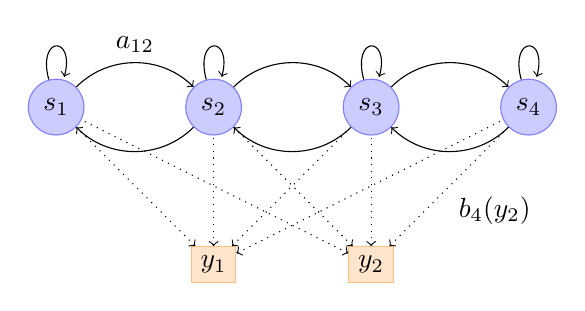
\begin{tikzpicture}[]
% states
\node[state] (s1) at (0,2) {$s_1$}
    edge [loop above]  ();
\node[state] (s2) at (2,2) {$s_2$}
    edge [<-,bend right=45] node[auto,swap] {$a_{12}$} (s1)
    edge [->,bend left=45] (s1)
    edge [loop above] ();
\node[state] (s3) at (4,2) {$s_3$}
    edge [<-,bend right=45] (s2)
    edge [->,bend left=45] (s2)
    edge [loop above] ();
\node[state] (s4) at (6,2) {$s_4$}
    edge [<-,bend right=45] (s3)
    edge [->,bend left=45] (s3)
    edge [loop above] ();
% observations
\node[observation] (y1) at (2,0) {$y_1$}
    edge [lightedge] (s1)
    edge [lightedge] (s2)
    edge [lightedge] (s3)
    edge [lightedge] (s4);
\node[observation] (y2) at (4,0) {$y_2$}
    edge [lightedge] (s1)
    edge [lightedge] (s2)
    edge [lightedge] (s3)
    edge [lightedge] node[auto,swap] {$b_4(y_2)$} (s4);
\end{tikzpicture}
\end{center}
\caption{An HMM with 4 states which can emit 2 discrete symbols $y_1$ or $y_2$.
$a_{ij}$ is the probability to transition from state $s_i$ to state $s_j$.
$b_j(y_k)$ is the probability to emit symbol $y_k$ in state $s_j$.
In this particular HMM, states can only reach themselves or the adjacent state.\ikN{Check wording, might be copy-pasted (reference source)}}
\label{fig:HMM}
\end{figure}







The HMM formed the definitive state of the art in the early 1990s \cite{rabiner1989tutorial}, with DSP hardware applications being sold in a market for office systems, manufacturing, telecommunications, and other areas \cite[p.487]{rabiner1993fundamentals}. 

%Prominent contributions \cite{rabiner1993fundamentals} (book, fundamentals of theory etc), [cite2]. The improvements came from the introduction of ... (better theoretical understanding?/more powerful hardware? more data?)


To improve the quality of feature representations that are used as inputs to the HMM, there was a shift to hybrid Deep Neural Network Hidden Markov systems (DNN-HMMs) from Gaussian Mixture Model HMMs (GMM-HMMs). GMMs in GMM-HMM systems have a serious shortcoming in that they are statistically inefficient for modeling data that lie on or near a nonlinear manifold in the data space \cite{hinton2012deep}. This is problematic as speech is inherently highly non-linear [cit]. DNN-HMM design follows traditional GMM-HMM systems. As the DNN is used to model the posterior probability of a state given an observation vector, a prior is required. The prior is commonly obtained with a Viterbi algorithm of the GMM-HMM approach and is given in the form of an initial labeled state sequence \cite{li2013hybrid}. In acoustic modeling for large vocabulary continuous speech recognition (LVCSR) tasks, DNN-HMMs were shown by Dahl et al. \cite{dahl2012context} to give significant gains over state-of-the-art GMM-HMM systems in a wide variety of small and large vocabulary tasks. Reductions in relative error of 16.0 \% and 23.2 \% were demonstrated using context-dependent DNN-HMMs over context-dependent GMM-HMMs. Additionally, it was found that DNNs gave much higher accuracy when large training datasets supported the greatly increased model capacity \cite{deng2014achievements}

In GMM-HMM systems the feature representation is hand-crafted by the user, typically in the form of Mel-frequency cepstral coefficients (MFCCs). The Fourier transform can be temporally windowed with a smoothing window function to create a Short-time Fourier transform (STFT). MFCCs create lower-dimensional representations by taking the STFT, applying a non-linear transform (the logarithm), pooling, and a final affine transform. 


 MFCCs, GMMs and HMMs co-evolved in speech recognition in an era with limited computational power. MFCCs lose significant information from the sound wave, but preserve higher order low-dimensional information that is required for discrimination. This is to partially overcome the very strong conditional independence assumptions of HMMs \cite{mohamed2012acoustic}, as well as improve tractability of the problem [cit?].
% \emph{MFCCs, GMMs, and HMMs co-evolved as a way of doing speech recognition when computers were too slow to explore more computationally intensive approaches. MFCCs throw away a lot of the information in the sound wave, but preserve most of the information required for discrimination. By including temporal differences, MFCCs partially overcome the very strong conditional independence assumption of HMMs, namely that successive frames are independent given the hidden state of the HMM. The temporal differences also allow diagonal covariance Gaussians to model the strong temporal covariances by reducing these particular pairwise covariances to individual coefficients.} 
%Could be bullshit: The hand-crafted phoneme representation front-end is replaced with ....
Whereas MFCCs led to significant accuracy improvements in GMM-HMM systems despite their known loss of information introduced, further advancements came from reducing the specificity of the signal transforms that were used to form feature representations.
For example, Mohamed et al. (2012a) \cite{mohamed2012acoustic} and Li et al., (2012) [cant find cit?] showed significantly lowered automatic speech recognition errors using large-scale DNNs when moving from the MFCC features back to more primitive (Mel-scaled) filter-bank features. The results implicated that DNNs are able to learn a better representation from Mel-scaled features than the final step of the MFCC transform: the discrete cosine transform. The original use of the cosine transform is justified by its approximate de-correlation of feature components. This is of importance to using diagonal covariance matrices with GMMs. This restriction however does not apply to deep learning models, as their strength in modelling data correlation makes the transform redundant. 

There is a possibility of future work to focus on training directly on raw waveforms, although current research has been unable to extract equivalent performance in audio applications, discussed further discussed at the end of Section \ref{sec:AED}.


%Names of subsections in paper (not sure what to use for): Better optimisation, architectures, transfer learning and noise robustness



%%%% Maybe re-instate later

% Historically, the use of rectified linear units to train large networks in computer vision carried over to training DNNs in speech detection, resulting in performance gains relative to DNNs trained with sigmoid units, with further improvement on GMM/HMM systems. \cite{dahl2013improving}
% \ikN{Find suitable place for the above point/remove}




HMMs suffer inherent limitations speech recognition applications. The assumption that successive observations are independent, as well as the probability of being in a state only depending on the state at the previous time step, do not strictly hold true \cite{rabiner1989tutorial}. The final major change in recent literature was the replacement of the HMM in its entirety, as well as the introduction of convolutional neural networks (CNNs) and Long short-term memory networks (LSTMs) for feature generation\ikn{Define here?}. In large-scale speech tasks, deep convolutional nets have been shown to significantly outperform DNN-HMM systems by Sainath et al. \cite{sainath2015deep}. Their method trialled a combination of salient features (logarithmically spaced Fourier coefficients and other features stacked into one vector as used in \cite{soltau2010ibm}) to train the CNNs.

Due to the relevancy to current research \ikn{Re-word} we address the following implementation details. Compared to fully end-to-end trained DNNs\ikn{Check claim}, CNNs capture translational invariance with far fewer parameters by averaging the outputs of hidden units in different local time and frequency regions. The CNNs and fully-connected DNNs used 1024 hidden units per fully connected layer with sigmoid non-linearities. The last layer is a softmax layer with 512 output targets. The 512 targets were determined as a result of clustering context-dependent GMM/HMM states. The authors note decreasing performance when increasing layer depth beyond 2. 
	%\item Full weight sharing: allowing multiple convolutional layers, encouraging deeper networks (c.f. limited weight sharing: limited to one convolutional layer)
	
	%\item Pooling in time with overlap can thought of as a way to smooth out the signal in time, another form of regularization.
 


Further improvement was found with the application of recurrent neural networks \cite{graves2013speech}. The authors noted at the time of publication in 2013 that while HMM-RNN systems had seen a recent revival, they did not perform as well as deep networks. As with Sainath et al., the authors favoured to train RNNs ‘end-to-end’ fully, instead of combining RNNs with HMMs. This approach allowed RNNs to exploit their larger state-space capacity and richer dynamics, as well as avoid using potentially incorrect alignments as training targets. The combination of Long Short-term Memory [cit, 11 in orig paper], an RNN architecture, with end-to-end training has proved especially effective for cursive handwriting recognition \cite{graves2008unconstrained,graves2009offline}. Graves et al. \cite{graves2013speech} have shown that combination of deep, bidirectional LSTM RNNs with end-to-end training gave state-of-the-art results in phoneme recognition, and note that the next step is to extend the system to large vocabulary speech recognition. A further proposed direction is to combine CNNs and deep LSTMs.

We note the authors use the same feature representation (mel-scaled coefficients, with their first and second derivatives and a few extras), and propose the investigation of moving towards autonomous learning of the feature space (as discussed in the Proposal in Section \ref{sec:proposal}).
\subsubsection{Relevance to our application?}
Speech recognition, whether it is predicting particular phonemes, or their sequences, requires predicting a dynamic signal that is highly nonstationary and embedded in noise. The field has strong transferability to general audio event recognition, and indeed methods developed in speech recognition have been applied as black-boxes with little modification to tasks such as bird recognition, which we discuss in Section \ref{sec:birdrecognition}.


\ikN{I think I have to talk about relevance to mosquito detection in particular}\srN{put in and make decision later - probably best in}


\section{Image recognition}
\label{sec:imagerecognition}
\subsubsection{State of art before deep learning}
\ikN{Describe briefly}
Deep learning methods in image recognition have strong parallels with deep learning methods in acoustics. This stems from the fundamental frequency representation currently in use with sounds--the spectrogram. A spectrogram representation is a two-dimensional matrix with intensity measurements as entries. This is equivalent to a black and white image representation. Due to the incredibly large and concentrated research efforts, as evidenced by the number of entries to a wide variety of image recognition tasks \cite{russakovsky2014imagenet,ILSVRC15}, a vast range of sub-fields in neural networks underwent incremental improvements. We structure this section by noteworthy changes in characteristics of the networks.

\subsection{Depth}
A primary driving factor of progress in deep learning has been network depth. This was first formally addressed by Simonyan and Zisserman by steadily increasing the depth of the network by addition of convolutional layers, while fixing the remaining parameters of the architecture. This was feasible due to the use of very small convolution filters in all layers \cite{simonyan2014very}. The effect was to increase model complexity by allowing more non-linearities, and hence make the decision function more discriminative. Without spatial pooling in between convolutional layers, two $3 \times 3$ layers have an effective receptive field size of a single $5 \times 5$ layer. In addition, this results in a decrease of parameters (with an 81 \% reduction when replacing a $7 \times 7$ receptive field with three $3\times3$ layers). As a result, in addition to accuracy improvements, faster gradient back-propagation and hence training times were also achieved. This trend has continued in ILSVRC submissions, with winners of the [...] challenge consisting of CNNs with depth [5,16,32, and finally 152].


% Up to 2014:
% \cite{simonyan2014very}:
% \emph{Convolutional networks (ConvNets) have recently enjoyed a great success in large-scale image
% and video recognition (Krizhevsky et al., 2012; Zeiler \& Fergus, 2013; Sermanet et al., 2014;
% Simonyan \& Zisserman, 2014) which has become possible due to the large public image repositories,
% such as ImageNet (Deng et al., 2009), and high-performance computing systems, such as GPUs
% or large-scale distributed clusters (Dean et al., 2012). In particular, an important role in the advance
% of deep visual recognition architectures has been played by the ImageNet Large-Scale Visual Recognition
% Challenge (ILSVRC) (Russakovsky et al., 2014), which has served as a testbed for a few
% generations of large-scale image classification systems, from high-dimensional shallow feature encodings
% (Perronnin et al., 2010) (the winner of ILSVRC-2011) to deep ConvNets (Krizhevsky et al.,
% 2012) (the winner of ILSVRC-2012).
% With ConvNets becoming more of a commodity in the computer vision field, a number of attempts
% have been made to improve the original architecture of Krizhevsky et al. (2012) in a
% bid to achieve better accuracy. For instance, the best-performing submissions to the ILSVRC-
% 2013 (Zeiler \& Fergus, 2013; Sermanet et al., 2014) utilised smaller receptive window size and
% smaller stride of the first convolutional layer. Another line of improvements dealt with training
% and testing the networks densely over the whole image and over multiple scales (Sermanet et al.,
% 2014; Howard, 2014). In this paper, we address another important aspect of ConvNet architecture
% design – its depth. To this end, we fix other parameters of the architecture, and steadily increase the
% depth of the network by adding more convolutional layers, which is feasible due to the use of very
% small (3×3) convolution filters in all layers.}




% From 2015:



% From DeepID3: Face Recognition with Very Deep Neural Networks:``Using deep neural networks to learn effective feature
% representations has become popular in face recognition
% [12, 20, 17, 22, 14, 13, 18, 21, 19, 15]."

\subsection{Residual learning}
A recent advancement was presented by He et al. \cite{he2016deep} as deep residual learning. Their submission resulted in first place placements on ImageNet detection, ImageNet localization, COCO detection, and COCO segmentation in ILSVRC \&
COCO 2015 competitions. The authors argue that the breadth of categories in which excellent results are achieved is strong evidence that the method is applicable in other vision and non-vision problems. 
\ikN{Need link here e.g. The causal mechanics are explained by the author as follows...}
The authors define $\mathcal{H}(x)$ as an underlying mapping to be learnt by a few stacked layers of the network, with $x$ denoting the inputs to these layers. The authors argue that ``if one hypothesizes that multiple nonlinear layers can asymptotically approximate complicated functions, then it is equivalent to hypothesize that they can asymptotically approximate the residual functions, i.e., $\mathcal{H}(x) - x$". Instead of approximating $\mathcal{H}(x)$, the equivalent layers are approximating the residual function $F(x) := \mathcal{H}(x) - x$. The original function thus becomes $F(x)+x$. 

As a result, the mathematically equivalent formulations can be implemented with architecture modifications via identity mappings \cite[figx]{he2016deep}. The improved rate of learning deep architectures under this formulation allows the use of extremely deep networks. The 152-layer residual network was at the time of submission the deepest network ever presented at ImageNet, while still having lower complexity than VGG proposed in \cite{simonyan2014very}. The improvement is in line with the philosophy discussed in the previous sectio/by Simonyan and Zisserman.


\subsection{Data augmentation}
The prominent applications where neural networks significantly outperformed other means of classification all involved large datasets. Since its inception in 2009, the CIFAR10/100 dataset \cite{krizhevsky2009learning} served as an extremely useful testbed with over 1000 citations at the time of writing. The set contained 60,000 labelled samples, which were split into either 10 or 100 classes. At this date, since its introduction in [?] ImageNet contains over 14 million images, of which over a million come with bounding box annotations. For details of the ImageNet construction the interested reader is directed to \cite[Section 3]{ILSVRC15}, which discusses the crowdsourcing strategy for its three categories: image classification, single-object localisation, and object detection. Simonyan and Zisserman \cite{simonyan2014very} attribute much increase in performance due to computational hardware (GPU computing) and dataset availability. However with scarce data, and even with healthy datasets, it has been common practice to generate additional training data by applying transformations to the original data \cite{hinton2012improving}. The practice can be traced back to \cite{simard2003best}, where the authors note that synthesising plausible transformations of data is simple, however learning transformation invariance by a model can be arbitrarily complicated. If the data is both scarce, and the distribution to be learned has transformation-invariance properties, generating additional data using transformations may improve performance. Indeed this practice has become widely adopted in the neural network literature, with common transformations including translations, horizontal reflections, as well as warping functions [cit warp?]. In addition, modifications to intensities of RGB channels in training images \cite{krizhevsky2012imagenet} have been applied (similar to synthesising and adding various noise profiles for acoustics). The authors note that the transformations artificially increase the dataset size by over a factor of 2048 for the affine transformations alone. Despite the high inter-dependence of samples, the augmentation offers a form of normalisation, allowing the use of deeper networks while avoiding overfitting. As established, depth plays an important role in overall performance, which places great emphasis on producing as large of a training data set as possible. The augmentation has become common practice as evidenced in ILSVRC submission winners throughout the years \cite[check 3rd ref]{simonyan2014very,he2016deep,krizhevsky2012imagenet}.\ikN{Maybe link to proposal of data augmentations. Note also, this was performed in BirdCLEF}




\subsection{Deep Kernel Learning}
\ikN{Find a way to integrate this section properly}
To gain insight into understanding deep learning models, a less established practice that is gaining traction in recent years, is to view CNNs and other network configurations as instances of Gaussian Processes, or other kernel-learning methods [could be BS, find cit,cit,cit]. In transition to fully probabilistic models, some works attempt to build hybrid neural network/Gaussian process models to retain the performance benefit of deep learning methods, while also conforming to probabilistic predictions. Wilson et. al \cite{wilson2016deep} showed that jointly learning deep kernel parameters has advantages over training a GP applied to the output layer of a trained deep neural network. In addition, the jointly learned model outperformed the equivalent deep neural network, as well as more primitive CNN/DBN-GP combinations, on the MNIST dataset. The work forms the basis of a medium-term proposed goal addressed in Section \ref{sec:proposal}.


\srN{point out that only very recently have techniques from image analysis come into the signal world}
\subsection{Transferability}
Despite immense popularity in image recognition, until recently there were relatively few convincing applications in signal processing. Similarly to how handcrafted scale-invariant features, Difference of Gaussians, and Histograms of Oriented Gradients [cit,cit,cit] were phased out with deep learning, handcrafted feature descriptors are beginning to undergo the same fate in acoustic signal processing. We illustrate this in Section \ref{sec:birdrecognition} with a bird recognition case study equivalent to ILSVRC. We further support this claim by reviewing advancements in the general field of acoustic event detection in Section \ref{sec:AED}.






\section{Bird recognition}
\ikN{Could combine with AED section and use subheadings like in Image Recognition}
\label{sec:birdrecognition}
A prominent example of the recent shift in methodology towards deep learning is the BirdCLEF bird recognition challenge. The challenge consists of the classification of bird songs and calls into up to 1500 bird species from tens of thousands of crowd-sourced recordings. The introduction of deep learning has brought drastic improvements in mean average precision (MAP) scores. The highest MAP score of 2014 was 0.45, achieved by combining two main categories of features for classification: parametric acoustic features consisting of spectral features, cepstral features, energy features and voicing-related features, and probabilities of species-specific spectrogram segments \cite{goeau2014lifeclef}. The feature sets were used in combination with unsupervised dimensionality reduction to train randomized ensemble decision trees. The runner-up used an MFCC feature foundation, with further PCA whitening, to train random forests (a full pipeline is given in Figure 3 in \cite{stowell2014automatic}).

Participants in the following year of 2015 achieved slightly lower scores due to the increased difficulty of the task \cite{goeau2015lifeclef}, with the best results achieved in very similar \ikn{Mention that same candidate} fashion to the previous year. However, 2016 marked the introduction of deep learning methods to the competition. Overall MAP scores improved to 0.69, outperforming the previously dominant method, which scored 0.58 on this occasion following small tweaks \cite{joly2016lifeclef}. The impressive performance gain came from the utilisation of well-established convolutional neural network practice from image recognition. By transforming the signals into windowed Fourier transform segments (forming a spectrogram with the Short-Time Fourier Transform  or STFT\ikn{Maybe expand point?}), the training data is represented by 2D matrices analogous to single-channel image representations. Following median-based segment de-noising, the authors employed a 5-layer CNN network on input sections of approximately 3 seconds in length. This allowed capturing and encoding the temporal dependencies of repeating birdsong or call patterns. The authors also noted no performance benefit from using 1D convolution with height equal to spectral width (frequency). As with common practice in image recognition, data augmentation was performed in the form of noise injection. We note that the implementation, while effective, was unremarkable compared to state of the art submissions of recent years seen in ILSVRC, so there may be further room for improvement. Coupled with the scarcity of overall submissions, there is strong evidence of a lack of maturity in this particular research area, which is expected to advance rapidly since the arrival of deep methods and over-saturation of submissions to image analysis challenges[cit?].


\section{Acoustic Event Detection}
\label{sec:AED}
To draw further parallels to our application\ikn{address explicitly}, we study recent research in Acoustic Event Detection (AED). This is the field that deals with detecting and classifying non-speech acoustic signals, with intent to convert continuous signals into a sequence of event labels associated with start and end times \cite{espi2015exploiting}. In recent years the field has attracted more research effort, with the foundation of dedicated challenges such as such as CLEAR \cite{mostefa2007chil}, and D-CASE \cite{giannoulis2013detection}, which involve detecting a known set of acoustic events indoors.


%AED applications range from rich transcription in speech communication \cite{mostefa2007chil,giannoulis2013detection} and scene understanding




The increased attention to deep learning methods can be evidenced at the Music Information Retrieval Evaluation eXchange (MIREX). Amongst many, example tasks include recognising musical chords, tempos, and genres \cite{mirex2016}. The majority of challenges require detecting a specific composition of frequencies localised in time. For instance, classifying musical instruments that play identical notes requires detection of the harmonic structure of the tones produced. This is analogous to many real-world problems, as the ratios of amplitudes of harmonics define particular sounds. Correct detection could allow discrimination of information-bearing harmonic stacks from background noise occurring at the same fundamental frequency. For example, the task may be to identify an insect flying in a room with constant noise produced by a fan at the same fundamental frequency. As part of our candidate challenge of accurately detecting mosquitoes in our paper [ref], this case was evidenced in our collected training data.\ikN{Making specific reference to mosquito detection but nowhere else?}
A meta-analysis of MIREX concluded that the state of the art stagnated in a variety of such classification and detection tasks (Humphrey et al. \cite{humphrey2013feature}) between 2007 and 2012. 
This was attributed to the use of traditional methods for feature extraction and classification. It was suggested deep learning can help overcome three deficiencies associated with traditional methods: 
\begin{enumerate}
    \item Hand-crafted feature design is not sustainable,
    \label{bullet:1}
    \item Shallow processing architectures struggle with latent complexity of real-world phenomena,
    \label{bullet:2}
    \item Short-time analysis cannot naturally capture higher-level information. 
    \label{bullet:3}
\end{enumerate}
Evidence for (\ref{bullet:1}) in this field was presented by Espi et al. \cite{espi2015exploiting}, who argue in favour of using more generic feature representations at the input layer of CNNs. This allows the network to truly exploit the feature learning ability of deep learning. Such claims are in line with the move to less complex features discussed in the speech recognition section(Section \ref{sec:speechrecognition}).
Indeed, since the assessment, there has been a paradigm shift. As an example, in 2016 challenge results \cite{mirex2016}, every (all-time) top performer in the four chord recognition challenges (Korzienowski, Widmer \cite{korzeniowski2016feature,mirex2016chord}) featured forms of deep networks operating on simple feature representations. Their contribution was the ability to discover feature representations from a basic frequency representation (the STFT or constant-Q transform) that were better suited to use with a conditional random field than hand-crafted representations. The authors note that hand-crafted representations benefited from using a further transform on the STFT (a logarithmic tiling by means of a constant-Q transform \cite{brown1991calculation}), whereas the neural network was insensitive to the base representation.


Further evidence for (\ref{bullet:1}) is presented by Espi et al. \cite{espi2015exploiting} in a meta-study of acoustic events. The authors noted that pooling, especially in frequency, seemed to degrade the network's ability to detect events. As a result, use of salient features (MFCCs) would result in worse overall performance than learning features with deep models directly from the spectrogram (STFT). Additionally, multiple time-frequency resolutions may be required to parameterise the STFT, which underpins a shortcoming of the windowed Fourier transform: a fixed time-frequency resolution. This shortcoming has been well-studied in the signal processing community, yet it is rare to find considerations of this at the intersection of acoustics-based deep learning research. Therefore we believe this warrants basis for further research, as addressed in the Proposal in Section \ref{sec:proposal}. For our application of mosquito detection we addressed this shortcoming in Section [ref] of the paper [ref].


Additional support for (\ref{bullet:1}) is presented by Phan et al. \cite{phan2016robust}, where the authors compare popular traditional classifier combinations to CNNs and DNNs. 
%Traditional feature-classification pairings studied included SVM + MFCC (and enhanced version of it), MPEG/PCA + HMM, Gabor + HMM, and MFCC + Gabor. SIF: spectrogram image features. 
With the use of variable convolutional filter sizes, relatively shallow networks with  1-max pooling strategies significantly outperformed traditional approaches on their given dataset across a range of SNRs. Strongest improvements where evidenced in low SNR scenarios, where traditional methods would fully break down. The signal data was obtained from the Real World Computing Partnership Sound Scene Database in Real Acoustic Environments. The authors attempted to minimise bias by randomly sub-sampling the dataset into  2000, 500, and 1500 event instances for training, validation, and testing purposes, respectively. 

Irrespective of finer details, a very clear benefit to CNNs over HMM/SVM combinations is evidenced with the introduction of noise. Additionally, there is a reliable benefit to CNNs over DNNs as consistent with speech recognition literature. Furthermore, a general trend for generic spectrogram features to be preferable to more salient features such as MFCCs and Gabor features was demonstrated with the use of CNNs. The CNN architecture was both simple and efficient. We note varying convolutional size filters were employed, that were learnt from data automatically. As often it is unclear over what time-scale events happen predictably exactly, this may be a highly useful feature to implement in future works.

% negatives:
% begin{itemize}
% 	\item Little gains over conventional CNN on SIF in clean signal scenario
% 	\item Little implementation detail given
% 	\item No hyperparam optimisation 
% \end{itemize}

% A further meta-review of the music informatics field \cite{humphrey2013feature} argues for the need to learn feature representations to take away the hand-crafted process of both choosing feature extraction methods, as well as classification algorithms. [Feature extraction has parallels to data compression: efficient learning of representations (also perhaps useful in replacing conventional audio codecs?)] A key point presented is that A good representation is sufficient for good overall performance, and it is important not to demand the impossible from the classifier \ikN{To self: see Non-linear semantic embedding vs PCA, with use of kNN pp.15-16)}

Further CNN proponents (and support for claim (\ref{bullet:3})) include the ability to better capture long-term information (dependence of sample on previous samples). In the limit an example is given in the WaveNet paper \cite{van2016wavenet} where each sample is conditioned on every preceding sample by using causal correlation filters. On the other hand, conventionally, features derived from short-time signals are limited to the information content contained within each segment. As a result, if some musical event does not occur within the span of an observation---a motif that does not fit within a single frame---then it simply cannot be described by that feature vector alone. This is in part addressed by the Markov property as regularly used in speech detection [see section above], but still imposes a limit on single-frame/sequence dependence [check exactly how dependence works].

%Deep Image Features in Music Information Retrieval
\ikN{Note that one may save resources by utilising transfer learning \cite[Paper uses a Caffe ILSVRC CNN as baseline]{gwardys2014deep}}


% \subsubsection*{Non-linear semantic embedding for instrument sample libraries \cite{humphrey2011non} \footnote{ieeexplore.ieee.org/iel5/6146696/6147038/06147663.pdf}}
% \begin{itemize}
% 	\item Traditional neural nets: spatial organisation of input vector inconsequential to network. Solved by use of CNNs: sensitivity to highly correlated data and varying degrees of translation invariance
% \end{itemize}





% \subsubsection*{Deep learning for detection of bird vocalisations \cite{potamitis2016deep}}
% \begin{itemize}
% 	\item Linked by Davide 

% 	\item Autoenconder, convolutional``U-net" (\url{http://lmb.informatik.uni-freiburg.de/people/ronneber/u-net/})
% 	\item Does not discriminate between species in current configuration
% \end{itemize}
	




\subsubsection{Learning a frequency decomposition}

Taking Humphrey's claim (\ref{bullet:1}) to the limit and to further facilitate autonomous behaviour, the next potential research challenge would be to operate on raw data, rather than raw ``spectrogram'' data, as alluded to by [cit cit cit]. Spectrogram representations are not ``raw'', as they require both a parameterised Fourier transform, as well as a smoothing window at a fixed resolution (or in some case multiple transforms at different resolutions to detect events occurring over differing time scales \cite{espi2015exploiting}) to construct.

While few papers have achieved noteworthy results in this field, Dieleman et al. \cite{dieleman2014end} show promising results in a range of music information retrieval tasks. The authors note that while raw performance of STFT methods was not matched, the networks were able to autonomously discover frequency decompositions from raw audio, as well as phase and translation-invariant feature representations. Furthermore, successful applications have arisen in raw audio \emph{generation} \cite{van2016wavenet}. The authors employed a .... architecture to synthesise speech and music sequences with remarkable results. A possible stepping stone towards moving towards fully autonomous feature extraction may be learning wavelet bases that suit the data [cit]. We address this in our research proposal, and demonstrate practical performance improvements in our paper [ref].




\begin{comment}

\subsubsection*{Steve}
Read through:
\begin{itemize}
	\item Bell: Edges are `Independent Components' of Natural Scenes. Note the emergency of wavelet-like  filters: DC filter, oriented filters and localised checkerboard patterns. Originated from an information theoretic learning rule which has no noise model and is sensitive to higher-order statistics.
	\item Aapo Hyvarinen
	\item Plumbley: `If the Independent Components of Natural Images are Edges, what are the Independent Components of Natural Sounds? Argument for ICA representation resembling layout of the auditory filter-bank in humans, equivalence to Bell's discovery in vision stated.
\end{itemize}
Consider:
\begin{itemize}
	\item Find paper (send to Steve) comparing wavelet to raw audio performance: have benefits been considered for combining information from both models or training on a vector containing both frequency and temporal representations?
	\item As on overall problem we are considering a function to maximise detection utility. An approach may be information theoretic -- wavelet-like structures appear (i.e. ICA) -- or stem from CNNs/RL: spectrogram vs raw data itself.
	\item Maximising information throughput in a system, ICA (commonly? or was?) used for pre-training lower layers in a network architecture
	\item Google paper: search for topic of: what is easy to classify, what isn't. Building a hierarchy successfully: solve easy parts first, rather than trying to solve everything at once and end up solving nothing
	\item When simulating data for training, consider if inverting our `generative' model can yield an optimal detector? Problems may include location invariance/pose/orientation not being captured, leading to issues with generalisation.
\end{itemize}



\subsection{Reading}
\subsubsection*{Deep Gaussian Processes}
\texttt{deeplimits.pdf}
\begin{itemize}
	\item Viewing deep neural networks as priors on functions. Can analyse their properties without reference to any particular dataset, loss function or training method.
	\item Deep Gaussian processes: compositions of functions drawn from GP priors
	\item Motivations:
	\begin{itemize}
		\item Damianou et al. showed the probabilistic nature of deep GPs guards against overfitting.
		\item Hensman et al. showed stochastic variational inference is possible in deep GPs, allowing mini-batch training on large datasets.
		\item Availability of approximation to marginal likelihood allows one to automatically tune the model architecture without the need for cross-validation.
	\end{itemize}
	\item Representational capacity of standard deep networks tends to decrease as number of layers increases?
	\item Propose alternate network architecture that connects input to each layer that does not suffer from this pathology.
	\item Conclusions:
	\begin{itemize}
		\item Existing neural network practice requires expensive tuning of model hyperparameters such as the number of layers, the size of each layer, and regularization penalties by cross-validation. One advantage of deep GPs is that the approximate marginal likelihood
allows a principled method for automatically determining such model choices.
	\end{itemize}
\end{itemize}


\end{comment}





\begin{comment}
\subsubsection{Learning stationary time series using Gaussian processes with nonparamteric kernels}
Replace human element of searching for kernels. The human element undesirable as:
\begin{itemize}
	\item Motivation
	\begin{itemize}
		\item Heuristic search unreliable
		\item Recent approaches automate search, mimicking the way in which a human would search for a best kernel
		\item Computational tractability limits complexity of kernels that can be designed in this way
	\end{itemize}
	\item Proposition
	\begin{itemize}
		\item Gaussian Process Convolution Model (GPCM). $$ f(t) = \int h(t-\tau) x(\tau) d \tau $$ $x(\tau)$ continuous white noise, draw from GP with delta-function covariance. $h(t)$ draw from a GP with some covariance function $K_h(t_1, t_2)$
	\end{itemize}
\end{itemize}




\section{To take further}
Toy problem:
\begin{itemize}
	\item Simplest: Singer male or female?
	\item Simple: Classify: Does this section contain a saxaphone solo or not? Solo contains many training samples, what kind of accuracy can we get by classifying chunks? Can we improve this accuracy by drawing from a database of other saxophone samples?
	\item Classify whether songs belong to a certain album by same band? Train nets on frequencies/hand-crafted features?
\end{itemize}
HumBug:
\begin{itemize}
	\item Train mosquito classifier on wavelet/Fourier spectra directly as images? How much information lost in image representations? Do we have enough mosquito data to train CNNs/other appropriate NNs?
\end{itemize}
General:
\begin{itemize}
	\item Theano tutorial
\end{itemize}
\end{comment}




% \section{Traditional Classification}
% \label{sec:traditional}

% Primitive methods: simple filters, extended to filterbanks: origin from digital electronic instrumentation



% Perhaps structure by application, talk about traditional -> deep learning. OR, collate fields and talk traditional -> deep learning with paragraphs/subsections for each application.



\section{Proposal}
\label{sec:proposal}
\subsection{Completed Work}
Our completed work presents an application of deep learning for acoustic event detection in a challenging, data-scare, real-world problem. Our candidate challenge was to accurately detect the presence of a mosquito from its acoustic signature. We developed convolutional neural networks (CNNs) operating on wavelet transformations of audio recordings. This was accomplished with the aid of a continuous wavelet transform with the bump mother wavelet -- a popular choice in traditional time-frequency analysis methods in signal processing [cite]. Furthermore, we interrogated network predictive power by visualising the statistics of network-excitatory samples. The visualisations offered insights into relative informativeness of components in the detection problem. It was shown that the network correctly learned acoustic properties of the mosquito, rather than peculiarities of the recording (such as microphone noise). Detection was achieved with performance metrics significantly surpassing those of existing algorithmic methods, as well as marginally exceeding those attained by individual human experts. The existing algorithmic methods trialled included Support Vector Machines, Random Forests, Naive Bayes classifiers, and Gaussian processes.


\subsection{Further Work}
The proposal is structured by approximate timelines. We define short-term goals as targets to address in two to three months, medium-term as three to nine months, and long-term as over nine months.
\subsubsection{Short-term}
\begin{enumerate}
\item Following our work on mosquito detection with the use of wavelet-conditioned Convolutional Neural Networks, it is hypothesised that the wavelet transform is more effective than the STFT from an information-theoretic viewpoint. We wish to explore this hypothesis formally. 
\begin{enumerate}
\item If proven true, this may have a profound effect on the deep learning literature, where the baseline state-of-art method involves taking the STFT before further learning. A possible way to test this would involve taking a pre-trained network from a paper, repeating all the steps with both STFT as a baseline, as well as the wavelet transform.
\item In the abundance of data, if it turns out that deep networks automatically learn more salient representations neglecting the benefits of wavelets, there is still valuable research to be made for data-scarce scenarios. As applications in the real world often involve expensive data collection and labelling, we consider this research avenue worthy of pursuit. 
\end{enumerate}
Should benefits be demonstrated in either scenario, the focus of work will be to improve on computational efficiency of the CWT algorithm implementation. A suitable alternative may be to use a discrete wavelet transform (DWT) that can be executed at the same computational complexity as the FFT [cit needed].
\item A further short term goal involves utilising data augmentation for training neural networks. In our mosquito detection application data is very expensive, so being able to generate data probabilistically using a scaffold model may help scale performance for multiple species and remain competitive with traditional classification methods, even in extremely data-limited scenarios. \ikN{look into GANs, also consider that we could generate representative samples from our network. Maybe we can make use of those to create new data}
\srN{this is a good idea and would really help alleviate the poverty of some data}

\item Our current method uses a parameterised wavelet transform as feature space conditioning for neural network computations. As a short- to medium-term goal we wish to extend this by also learning wavelet (or other) feature representation spaces jointly with the the remaining network parameters. This involves learning a kernel for frequency transformations. 
\ikN{Link to litreview. As evidenced in trends in image, speech etc. tendency to learn fully end-to-end}


\end{enumerate}
\subsubsection{Medium-term}
\begin{enumerate}
	\item The first medium-term goal in line is to bring probabilistic reasoning to our detection schemes, while maintaining the impressive performance offered by deep learning approaches. A major downside with neural networks is the inability to obtain model uncertainty (using a softmax to get probabilities is not enough to obtain model uncertainty. See extension originally mentioned by Denker and LeCunn \cite{denker1991transforming}). The aforementioned does not however apply \ikn{Not sure if this is true} to neural networks trained with deep kernel learning \cite{wilson2016deep}. As part of deep kernel learning (DKL), kernel parameters are learnt jointly with neural network hyperparameters the authors. This allows more principled handling of uncertainty. \ikN{Adam: analogy with type-II MLE used for inferring hyperparameters: OK as it happens higher up the inference chain, i.e. not used to learn model parameters} The authors demonstrated that jointly learning all DKL parameters has advantages over training a GP applied to the output layer of a trained deep neural network. Furthermore\ikn{Move details to litreview?}, in a range of regression and classification tasks, the DKL (hybrid GP/CNN) outperforms the equivalent CNN, GP applied to a fixed pre-trained CNN, GP applied to a pre-trained DNN, and a GP solely. With availability of code, a simple medium-term milestone would be to apply a DKL method with our equivalent wavelet-conditioned CNN to the mosquito data available at that stage of the project. 
	\item A further medium-term goal is to work on automation of neural network architecture optimization. This would build on work by Swersky et al. \cite{swersky2014raiders} which utilises a Bayesian Optimisation kernel \cite{snoek2012practical} for conditional parameter spaces to infer model architecture and corresponding hyperparameters. In line with our short-term objectives to infer wavelet feature representations, we would also like to build upon the BayesOpt framework to include a mechanism for learning hyperparameters in hybrid wavelet-CNN networks.

\end{enumerate}
\subsubsection{Long-term}
\begin{enumerate}
	\item In the long-term we wish to extend DKLs to our model which we will develop to jointly infer wavelet feature representation spaces and neural network parameters.
	\item The ultimate long-term goals are to build a dynamic detector that is able to also respond to changes in its environment. This is particularly relevant to signal detection over traditional image detection, as [change in stimulus in time-series compared to static image representations]. As part of the adaptability, the algorithm is required to recognise when the model is insufficient for explaining novel data. This may be incorporated using feedback mechanisms by drawing from ideas in evolutionary algorithms \cite{coello2007evolutionary}. We may wish to feed back uncertain results to a crowdsourcing platform to aid with creating a lifelong learning algorithm.
\end{enumerate}



\subsection{Risk Assessment}
We provide a risk assessment to identify critical points or uncertainties, and indicate how we will manage these. The assessment is categorised by high, medium and low risks, as well as their impact factors. For low-level risks we consider only those of high impact.

\subsubsection{High-level risks} 
\begin{enumerate} 
\item High impact: Benefit to using wavelets may have been purely due to saliency of feature, in particular the logarithmic tiling of the time-frequency plane, working well for small datasets
\item Medium impact: Advances in deep learning rendering our classification algorithms obsolete
\item Low impact: Changes in data acquisition rendering algorithm impractical or irrelevant (affecting the need to port/research efficiency of algorithms/DWT alternative)


\end{enumerate}


\subsubsection{Mitigating measures}
\begin{enumerate} 
    \item Research why performance benefit was shown for small datasets, and investigate CNN performance relative to other salient features. The CNN was trialled with a set of salient features, which were shown not to increase performance, so it is unlikely that only the saliency is responsible for the boost in performance when combining CNNs with the wavelet transform.
    \item This would not discredit our scientific contribution, but would affect practical implementations of algorithms on portable devices. This has a greater effect on the outcome of the HumBug project, but not on the PhD. A further mitigation measure is to combine advances in the field with our own advances.
	\item As with (2), this affects practical implementations. We could shift our focus to applications with dataset availability to suit our research needs, or adapt the algorithms to match new data availability. In the case of neural networks, this would involve adding further layers and model complexity without overfitting according to the new data size constraints.

\end{enumerate}

\subsubsection{Medium-level risks} 
\begin{enumerate}
	\item High impact: Inability to reproduce impressive performance results of CNNs when working with deep kernel methods, or other probabilistic models
    \item Medium impact: Proposed tasks are not met by desired date
    \item Low impact: Inability to reproduce performance when working towards autonomous frequency representation discovery
\end{enumerate}
\subsubsection{Mitigating measures}
\begin{enumerate}
	\item Work towards a hybrid probabilistic neural network model to leverage gains in both fields
    \item Set regular milestones and consider conference deadlines to focus work towards a specific scientific contribution
    \item Not necessarily a problem, as currently publishing with raw data methods is accepted with poorer performance, as long as an original scientific contribution is made \cite{dieleman2014end}.
\end{enumerate}

% \subsubsection{Low-level risk} 
% \begin{enumerate}
% 	\item High impact: 
% \end{enumerate}

\section{Conclusion}
\label{sec:litreviewconclusion}
Paradigm shift from hand-crafted to DNN to CNN. Image analysis moving towards RNNs/hybrid LSTM/CNN. Work seeing CNNs as deep kernel methods. Our target for future research. Furthermore, all signal detection performed in frequency domain with simple STFTs, we can use a more general transform with wavelets [need something about wavelets in lit review]. Perhaps there is a move towards raw data: unlikely to happen in future x years because [evidence of poor raw performance, despite small success stories]. Deepmind finds a way to get stuff to work where it doesn't make sense. Non-intuitive methodology, unclear how architectures came to light etc.




\bibliography{TransferBib}




\end{document}